\scanpage{44}
precisely, we have in addition an increasing and continuous map
\[
(2^\circ)\quad (\unsure{1|2}5)\qquad \Sigma_*\longrightarrow I
\]
(whence
\[
\Sigma_*=\coprod_{i\in I}\Sigma_i\ ,\quad
\Sigma_{**}=\underset{i\leq j}{\deleted{\sum}\inserted{\unsure{\coprod}}}\Sigma_{ij})
\]
\deleted{\unsure{with} $\Sigma_{ii}\simeq\Sigma_i$)}

\margin{\begin{tabular}{@{}l@{\;}l@{}}Condition \textcircled{a}&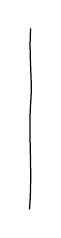
\begin{tikzpicture}[x=1cm,y=1cm,baseline=(current bounding box.center)]\draw[line width=.45pt] (0,0) .. controls (-.025,-.35) and (.025,-.65) .. (0,-.95) .. controls (-.03,-1.35) and (.025,-1.8) .. (-.015,-2.3);\end{tikzpicture}\end{tabular}}
And we \deleted{\unsure{require}} suppose that $\forall i,j$, \begin{tabular}[b]{@{}l@{}}\inserted{$i\leq j$}\\[-.8ex]\begin{tikzpicture}[x=1cm,y=1cm]\draw[line width=.4pt] (.6,.25) .. controls (.3,.15) and (.1,.1) .. (0,0);\end{tikzpicture}\end{tabular} the target morphism
\[
\Sigma_{ij}\unsure{-|\longrightarrow}\Sigma_j
\]
is a \deleted{\unsure{immersion|immersion}} \begin{tabular}[b]{@{}l@{}}\inserted{``cylindrical''}\\[-.5ex]\begin{tikzpicture}[x=1cm,y=1cm]\draw[line width=.4pt] (0,0) .. controls (-.05,.2) and (.1,.34) .. (.4,.34) -- (1.6,.34) .. controls (1.82,.34) and (1.9,.43) .. (1.85,.57);\end{tikzpicture}\end{tabular} closed embedding -- which implies (by injectivity) that (25$^*$) has the property that if $z\in\Sigma_*$ lies over $j$ and if $i\leq j$, then there exists \uline{at most} one $y\in\Sigma_*$ \unsure{\deleted{lying}|lying} \unsure{over|under} $i$, with $y\leq z$.
\margin{\unsure{i.e.|via} $\Sigma_*^{\leq z}\longrightarrow I^{\leq j}$ \unsure{injective}}

This also implies
\[
(26)\qquad\Sigma_{ii}=\Sigma_i
\]
\margin{\begin{tabular}{@{}l@{\;}l@{}}\deleted{condition \unsure{b)}}&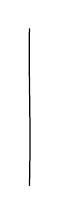
\begin{tikzpicture}[x=1cm,y=1cm,baseline=(current bounding box.center)]\draw[line width=.45pt] (0,0) .. controls (-.015,-.5) and (.02,-1.1) .. (0,-2);\end{tikzpicture}\end{tabular}}
\unsure{For|We} \deleted{\unsure{suppose} moreover that for $z\in$} \deleted{$\unsure{i}\unsure{\leq|<}j\unsure{\leq|<}k$,}
\[
(27)\qquad \Sigma(n)=\text{set of strict flags of length }n\text{ of }\Sigma
\]
\deleted{$\Sigma_i$}
\unsure{or|and}
\[
(27)\qquad
\begin{aligned}
\Sigma(n)&\longrightarrow\deleted{\unsure{I|\Sigma}}\operatorname{Drap}_n(I)\quad\text{(}\unsure{\text{strict flags|strict flags}}\unsure{)}\\
\Vert\quad&\\[-1ex]
\coprod_{\substack{(i_0<<i_n)\text{ strict flag in}\\ I\text{ of length }n}}\Sigma_{i_0- i_n}&
\end{aligned}
\]
\margin{OK}
\margin{\unsure{thus allows the statement} of condition (\unsure{b})}
\margin{43}
